\documentclass[a4paper]{ctexart}
\usepackage{xeCJK}
\usepackage{setspace}
\usepackage{graphicx,wrapfig}
\usepackage{fontspec,xunicode,xltxtra}
\usepackage{fancyhdr,titlesec,titletoc}
\usepackage[titletoc]{appendix}
\usepackage[top=29mm,bottom=29mm,left=31.8mm,right=31.8mm]{geometry}
\usepackage{enumerate,enumitem}
\usepackage{caption}
\usepackage{amsmath,amssymb,bm,array}
\usepackage{cite}
\usepackage{diagbox}
\usepackage{algorithm,algorithmicx,algpseudocode}
\usepackage{multirow}
\usepackage[super]{gbt7714}
\setmainfont{Times New Roman}
%\setCJKmainfont{SimSun}
\setCJKfamilyfont{heiti}{SimHei}
\renewcommand{\heiti}{\CJKfamily{heiti}\fontspec{Times New Roman}}

\newcommand{\mycaptionfont}{\heiti\zihao{5}}
\captionsetup[figure]{name={\mycaptionfont 图},labelsep=period}
\captionsetup[table]{name={\mycaptionfont 表},labelsep=period}
\floatname{algorithm}{\mycaptionfont 算法}
\captionsetup[algorithm]{labelsep=period}
\renewcommand{\captionfont}{\mycaptionfont}
\renewcommand{\captionlabelfont}{\mycaptionfont}

\ctexset {
	section = {
		number = \arabic{section},
		format = \zihao{4}\bfseries,
	},
	subsection = {
		number = \arabic{section}.\arabic{subsection},
		format = \zihao{-4}\bfseries,
	},
	subsubsection = {
		number = \arabic{section}.\arabic{subsection}.\arabic{subsubsection},
		format = \zihao{-4}\bfseries,
	}
}
\setlist[enumerate]{itemindent=2em,listparindent=2em,leftmargin=0em,label=\arabic*、}

\setlength\parskip{.5\baselineskip}
\fancypagestyle{plain}{\pagestyle{fancy}}%改变章节首页页眉
\pagestyle{fancy}
\lhead{\kaishu~人工智能课程作业~}
\rhead{\kaishu~1030616134~尹达恒}
\cfoot{\thepage}

\renewcommand{\abstractname}{摘要}
\renewenvironment{abstract}{
	\quotation
	\begin{spacing}{1.2}
		\par\zihao{5}{\bfseries \abstractname:}
	}{\end{spacing}\vskip 2.5ex}

\begin{document}
\begin{center}
	{\zihao{-3}\textbf{面向实时交互式视频通信流量调节的客户端智能Agent设计和关键技术}}

	{\zihao{-4}尹达恒}\\[-1mm]

	{\zihao{5}(东南大学,江苏\quad 南京)}
\end{center}
\begin{abstract}
	待定待定待定待定待定待定待定待定待定待定待定待定待定待定待定待定待定待定待定待定待定待定待定待定待定待定待定待定待定待定待定待定待定待定待定待定待定待定待定待定待定待定待定待定待定待定待定待定待定待定待定待定待定待定待定待定待定待定待定待定待定待定待定待定待定待定待定待定待定待定待定待定待定待定待定待定待定待定待定待定。

	\textbf{主题词:} 策略,流量调节,联邦学习,强化学习,机器学习
\end{abstract}
\renewcommand{\baselinestretch}{1.3}
\zihao{5}

\section{场景描述}

2020年的新冠肺炎疫情对传统的面对面“接触式”办公模式带来了巨大的冲击,作为“无接触式”办公模式的重要组成部分,视频会议软件得到的空前的发展,实时交互式视频通信应用迅速渗透到各行各业的生产活动中。

根据Cisco发布的年度网际网络报告(Cisco Annual Internet Report)\cite{CiscoAnnualInternetReport},在当今的所有互联网流量中,实时交互式视频流量占据着主导地位。随着LTE-Advanced和5G的发展,新的低延迟应用也在迅速出现,例如实时视频/VR广播、云游戏、手术机器人或车辆的远程操作等。这样的交互式视频应用比视频会议应用在带宽和延迟方面的要求更加苛刻。尽管电信基础设施努力满足需求,但基础设施仅能提供尽力而为的服务,因此,为了适应高度动态的网络条件和不同应用场景多样化的需求,在交互式视频通信客户端一侧的流量调节必不可少。

\begin{enumerate}[label=\arabic*、]
	\item 应用领域:交互式视频通信;
	\item 主要功能:在客户端一侧,根据网络环境实时地调节流量策略。
\end{enumerate}

\section{智能化任务}

在上述在交互式视频通信客户端一侧调节流量的应用场景中,人工智能算法需要处理的智能化任务可以概括为:

\begin{itemize}
	\item 输入:算法要能够及时地获取客户端一侧当前网络情况;
	\item 输出:算法要需要根据获取到的网络情况调节视频编码的比特率;
	\item 优化目标:视频编码的比特率应该调节到恰好使网路不发生拥塞。
\end{itemize}

\section{任务环境分析}

智能Agent的任务环境图\ref{figure:env}所示。本节将从Agent的输入输出和优化目标出发对Agent的任务环境进行分析。

\begin{figure}[htbp]
	\centering
	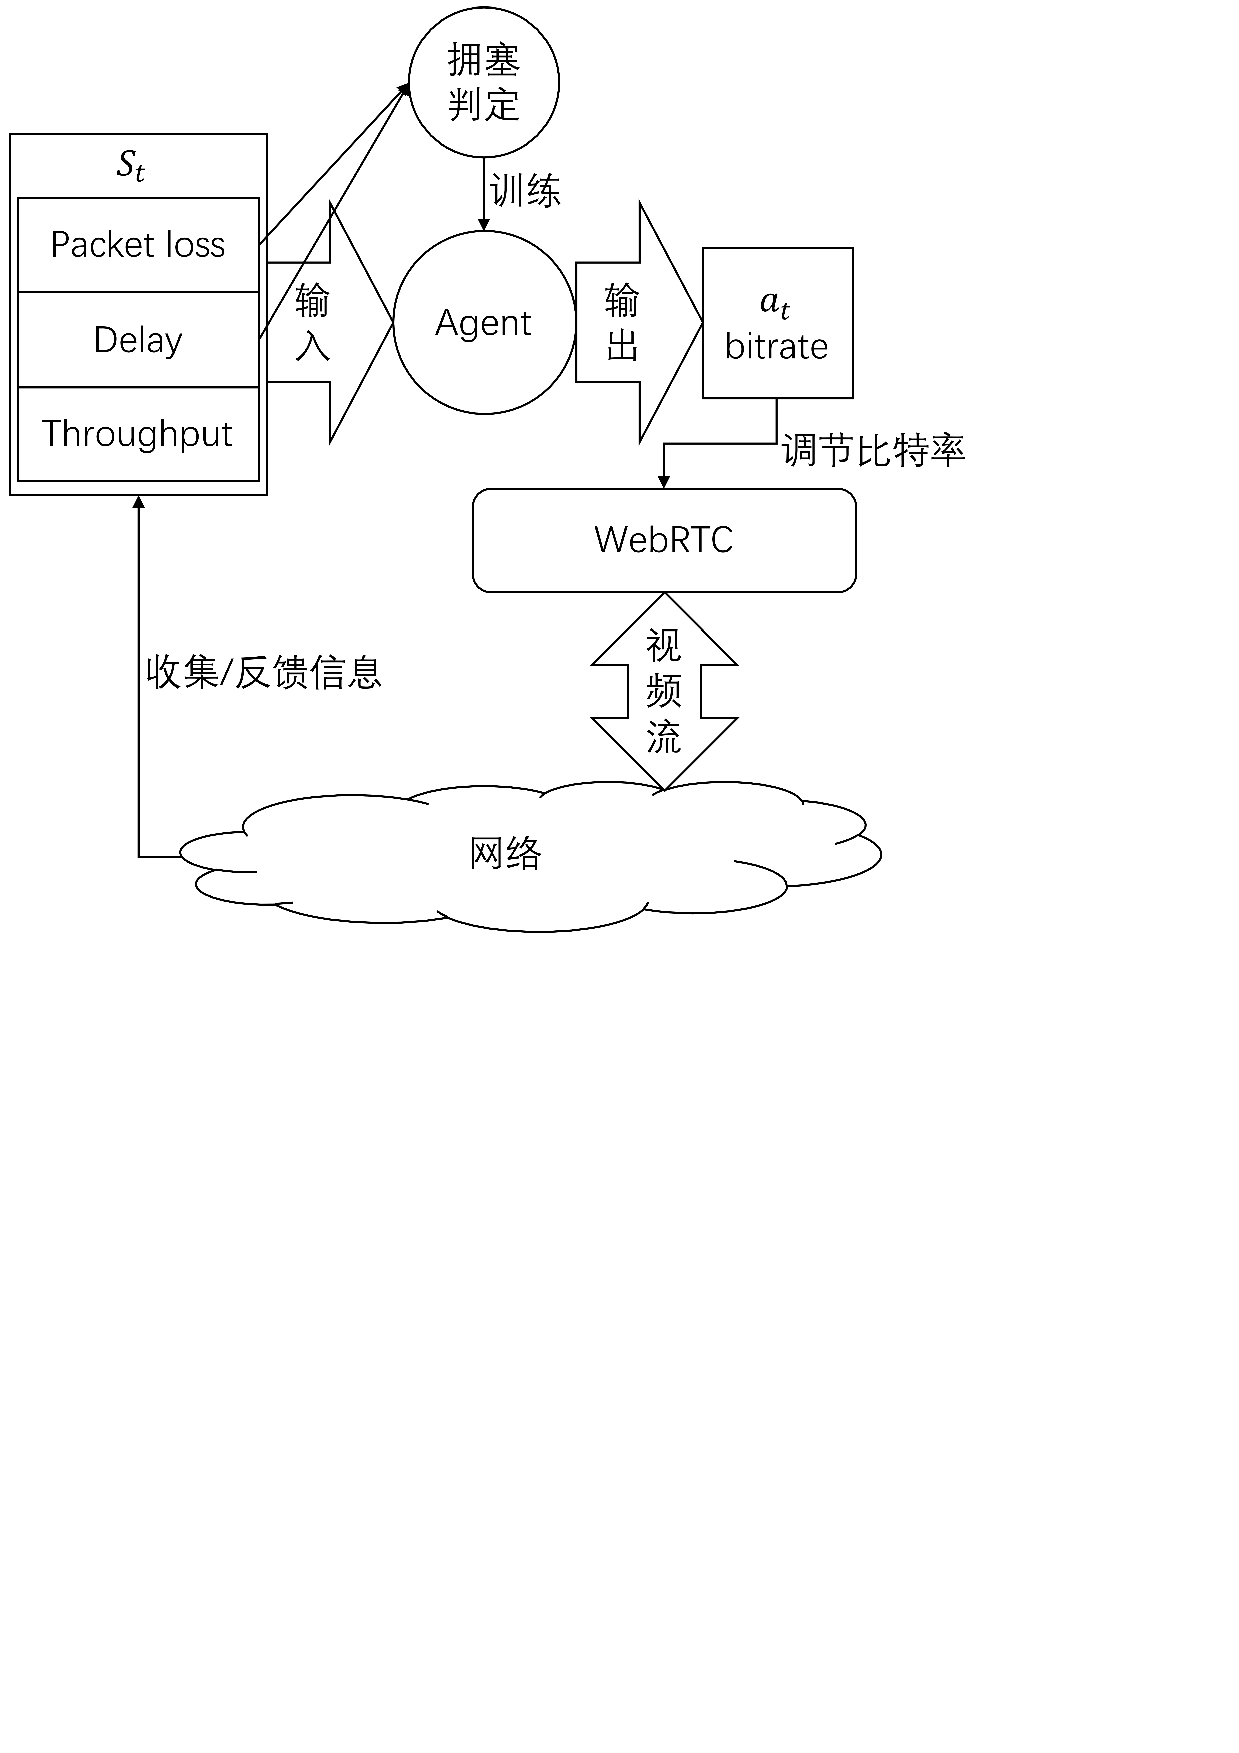
\includegraphics[width=0.9\textwidth, keepaspectratio]{figure/env.pdf}\\
	\caption{智能Agent的任务环境}\label{figure:env}
\end{figure}

\subsection{Agent输入分析}

网络情况所涵盖的变量很多,但大部分变量都记录在路由器、交换机等运营商侧的设备中。显然,实际情况下,运营商不可能在机房中大面积部署高能耗的人工智能应用,也不大可能将通信设备的状况信息开放给用户获取。因此,在客户端侧,Agent所能获取到的信息是比较有限的。根据目前交互式视频通信所使用的TCP/IP协议的内容,Agent可以获取到如下的网络状况信息:

\begin{enumerate}[label=\arabic*、]
	\item 丢包率(Packet loss):根据TCP协议中的超时重传规则,在TCP协议中对正常发送的包和重传包进行计数,即获取一定时间内的丢包率信息;
	\item 延迟(Delay):根据TCP协议的ACK机制,对包发送完成和收到确认ACK的时间间隔进行计数,即可获得发送过程的延迟信息;
	\item 吞吐量(Throughput):根据TCP协议中的发送机制,对一定时间内所有成功发送和解释到的包的大小进行求和,即可获得吞吐量信息。
\end{enumerate}

令$S_t=(Packet loss,Delay,Throughput)$表示$t$时刻Agent输入的网络状况信息。

\subsection{Agent输出分析}

由于视频流需要连续发送的特点,在设计Agent时可以不必考虑包发送的时刻问题,而只用考虑一段时间内发送包的数据总量,即视频流的比特率。目前视频流应用常用的WebRTC框架即具有动态调节视频比特率的功能。

令$a_t$表示Agent对输入$S_t$给出的输出,即视频比特率。

\subsection{Agent优化目标分析}

根据TCP/IP协议的丢包规则,当网络发生拥塞时,数据包在设备中的排队时间将显著增大,网络中无法承载的数据包将被网络设备直接舍弃,在客户端一侧的表现就是丢包率和延迟的急剧增大。因此,如果Agent输出比特率$a_t$超过可用带宽,则将导致网络拥塞,进而在下一个状态$S_{t+1}$中出现较高的丢包率和较大的延迟。因此,通过观察从$S_t$到$S_{t+1}$的丢包率和延迟变化,就能判定网络是否出现拥塞,进而判定Agent输出的$a_t$是否合适。如果$a_t$超过可用带宽,那么当下次观察$S_t$或类似状态时,Agent应输出较小的$a_t$;反之,Agent应输出较大的$a_t$。由此,Agent可以逐步逼近恰好使网路不发生拥塞的视频流比特率。

\section{智能Agent结构}



给出适合的Agent结构,及具体模块的结构;
\section{问题}
\begin{enumerate}[label=\arabic*、]
	\item 如何适应动态的网络条件
	\item 大量的Agent在各自的硬件上独立地运行,如何进行训练
	\item 视频编解码器的调节具有滞后性
	\item 掌握机器学习分类算法的性能提升方法;
	\item 能编程实现一些机器学习分类算法并进行性能分析和改进;
	\item 了解人工智能和分类算法的新进展、新应用。
\end{enumerate}
\section{现状}
上述问题的已有解决方法及其优缺点分析;
在虚拟环境中训练
\section{技术分析}
给出采用一个课本中现成方法和算法的优缺点分析,结合上述优缺点分析,进一步给出本文的具体技术和算法方案;
\section{方案分析}
给出本文方案实际应用中的可行性分析。

具体来说,决策树的构建方法可以表示为算法\ref{alg:DT}\cite{RN90}。
\begin{algorithm}[htbp]
	\caption{\mycaptionfont 决策树学习的基本算法}
	\label{alg:DT}
	\begin{algorithmic}[1]
		\Require 训练集$\mathcal{D}=\left\{(\bm x_i,y_i)|1\leq i\leq m\right\}$、属性集$\mathcal{A}=\left\{a_i|1\leq i\leq d\right\}$
		\Ensure $\forall (\bm x_i,y_i)\in \mathcal{D}$,属性值$a_i(\bm x_i)$存在
		\Function {DecisionTree}{$\mathcal{D}$,$\mathcal{A}$}
		\If{$\mathcal{D}$中的样本全部属于同一类别$C$}
		\State \Return 单节点树,类别标记为$C$
		\EndIf
		\If{$\mathcal{A}=\varnothing$}
		\State \Return 单节点树,类别标记为$\mathcal{D}$中样本数最多的类
		\EndIf
		\State 计算$\mathcal{A}$中每个特征的信息增益(ID3算法)或信息增益比(C4.5算法),从中选择最优属性$a_{best}$
		\For{$a_{best}$的每一可能值$a_{best}^t$}
		\State 令$\mathcal{D}'=\left\{(\bm x_i,y_i)|a_{best}(\bm x_i,y_i)=a_{best}^t,(\bm x_i,y_i)\in \mathcal{D}\right\}$
		\If{$\mathcal{D}'=\varnothing$}
		\State 添加叶节点,类别标记为$\mathcal{D}$中样本数最多的类
		\Else
		\State 递归添加分支节点\Call{DecisionTree}{$\mathcal{D}'$,$\mathcal{A}$}
		\EndIf
		\EndFor
		\EndFunction
	\end{algorithmic}
\end{algorithm}

将这4个分类结果占测试集总量的比率共同呈现于表\ref{tab:混淆矩阵}中,所形成的2$\times$2矩阵就称为混淆矩阵(Confusion Matrix)。相比于分类正确率,混淆矩阵能反映有关分类器性能的更加具体的信息,是分类预测模型性能评价的常用指标。
\begin{table}[htbp]
	\setstretch{1.5}
	\centering
	\caption{混淆矩阵}
	\begin{tabular}{|c|c|c|}
		\hline
		\diagbox{预测值}{混淆矩阵}{真实值} & 正 & 负 \\
		\hline
		正                                 & TP & FP \\
		\hline
		负                                 & FN & TN \\
		\hline
	\end{tabular}
	\label{tab:混淆矩阵}
\end{table}

\subsubsection{确定缺失项处理方法}\label{sec:确定缺失项处理方法}
缺失属性项确定之后,接下来就需要确定各缺失项的处理方法。
首先使用R语言读取“diabetes.csv”的数据并对数据集中的数据缺失情况进行统计:
\begin{enumerate}
	\item 统计“diabetes.csv”中的数据总行数,得到结果768;
	\item 使用mice包中的md.pattern()函数统计数据集中的数据缺失情况,数据缺失情况统计表(表\ref{tab:缺失数据统计})。
\end{enumerate}
\begin{table}[htbp]
	\setstretch{1.5}
	\centering
	\caption{数据缺失情况}
	\begin{tabular}{|c|ccccc|}
		\hline
		\diagbox{数据点数量}{是否缺失}{列名} & Glucose & BMI & BloodPressure & SkinThickness & Insulin \\\hline
		392                                  & 否      & 否  & 否            & 否            & 否      \\
		1                                    & 是      & 否  & 否            & 否            & 否      \\
		140                                  & 否      & 否  & 否            & 否            & 是      \\
		1                                    & 否      & 是  & 否            & 否            & 否      \\
		4                                    & 是      & 否  & 否            & 否            & 是      \\
		2                                    & 否      & 否  & 是            & 否            & 是      \\
		192                                  & 否      & 否  & 否            & 是            & 是      \\
		1                                    & 否      & 是  & 否            & 否            & 是      \\
		26                                   & 否      & 否  & 是            & 是            & 是      \\
		2                                    & 否      & 是  & 否            & 是            & 是      \\
		7                                    & 否      & 是  & 是            & 是            & 是      \\\hline
		列缺失总量                           & 5       & 11  & 35            & 227           & 374     \\\hline
	\end{tabular}
	\label{tab:缺失数据统计}
\end{table}
\section{实验结果与分析}
\subsection{实验结果}
\subsubsection{最高精度算法结果}
\begin{itemize}
	\item 算法最高精度:87.2611\%
	\item 最高精度算法:人工神经网络,见\ref{sec:人工神经网络}节
	\item 算法参数:见\ref{sec:进行逻辑回归}节和\ref{sec:ANN实践}节
	\item 混淆矩阵:
	\begin{table}[htbp]
		\centering
		\setstretch{1.5}
		\caption{最高精度算法结果的混淆矩阵}\label{tab:混淆矩阵}
		\begin{tabular}{|c|c|c|}
			\hline
			\%&估计样本0&估计样本1\\
			\hline
			真实样本0&64.33&7.006\\
			\hline
			真实样本1&5.732&22.93\\
			\hline
		\end{tabular}
	\end{table}
\end{itemize}

\newpage
\subsection{实验结果分析}
\begin{enumerate}
	\item 由表\ref{tab:混淆矩阵}可以看出:
	\begin{enumerate}[label=\alph*)]
		\item 错误估计的样本中假正例率和假负例率基本保持平衡,说明该算法对于正例和负例的判定都有比较好的结果;
		\item 正确估计的样本中主要都集中于真负例,说明该数据集的正负例非常不平衡;
		\item 上面两个结论表明,该算法在一个正负例不平衡的数据集中训练得到了一个假正例率和假负例率基本保持平衡的分类器,说明该算法具有很好的鲁棒性。
	\end{enumerate}
	\item 由图\ref{figure:ROC曲线}、图\ref{figure:总体正确率}和图\ref{figure:网络总体正确率}可以看出:
	      \begin{enumerate}[label=\alph*)]
		      \item 逻辑回归模型在该数据集上的准确性要略高于神经网络模型,且Dropout和L2正则化能使得神经网络模型的准确性和稳定性都有一定程度的提升,这说明本次实验中建立的神经网络模型在数据集上已经出现了过拟合现象,也印证了Dropout和L2正则化对神经网络模型过拟合的抑制作用;
		      \item 在三种使用不同核函数的SVM分类算法中,使用较为复杂的径向基核和多项式核构造SVM的分类正确率都不及最简单的线性核SVM,表明所使用的数据集中数据分布结构比较简单,复杂的核函数并不能对SVM分类准确率的提升有帮助;
		      \item 两种决策树算法在不同预处理数据集上的预测正确率相差很大,这表明决策树算法是一种不稳定的分类算法,在实际使用时需要一些后剪枝算法进行辅助;
			  \item 高斯朴素贝叶斯算法在不同的预处理数据集上都有大致相近的正确率,表明基于贝叶斯的分类算法具有较好的稳定性;
			  \item Stacking集成学习在多次重复实验中具有最高的稳定性,随机森林和AdaBoost集成学习算法在不同预处理数据集上的结果要比两种决策树算法都更接近,且随机森林算法的正确率要高于两种决策树算法,表明集成学习策略能提高机器学习算法的鲁棒性和准确性。
	      \end{enumerate}
	\item 由图\ref{figure:数据集正确率}和图\ref{figure:网络数据集正确率}可以看出:
	      \begin{enumerate}[label=\alph*)]
		      \item 经过EM填补的训练集训练出的机器学习算法在测试集上的准确率较为接近,且该训练集训练出的逻辑回归与神经网络算法在该测试集上的结果波动较小,表明EM填补相对于其他方法填补得到的训练集具有更好的分类特征,且不会与原数据集产生较大差异,对于有缺失数据的数据集使用EM算法能在一定程度上有提高训练出的机器学习算法的稳定性;
		      \item 删除“SkinThickness”列后的训练集训练出的逻辑回归与神经网络算法的测试集正确率较高但是波动很大,表明SkinThickness列并非是和糖尿病直接相关的特征,但是在一定程度上有助于糖尿病诊断;
		      \item 当删除训练集“Insulin”列或是“Insulin”和“SkinThickness”列都被删除时,逻辑回归与神经网络算法的测试集正确率都有所下降,这表明胰岛素确实时糖尿病诊断的重要特征。
	      \end{enumerate}
\end{enumerate}

\bibliography{ref}
\end{document}